\documentclass[../em.tex]{subfiles}
\graphicspath{{\subfix{../figures/}}}
\begin{document}
\chapter{Magnetic Fields and Electromagnetism}
\section{Magnetic Fields}
A magnetic field is a vector field that can be used to determine the magnetic force exerted 
on moving electric charges, electric currents or magnetic materials.
\begin{itemize}
    \item Produced by magnetic dipoles or combinations of dipoles, but never by monopoles.
    \item Magnetic dipoles have north and south polarity.
\end{itemize}

A magnetic field can be represented by using vector field maps.

Magnetic field lines must form closed loops, as described by Gauss's law of magnetism.
\begin{itemize}
    \item Gauss's law of magnetism is Maxwell's second equation.
    \item $\oint \vec{B} \cdot \dd\vec{A} = 0$
\end{itemize}

Magnetic dipoles results from the circular of rotational motion of electric charges.

A magnetic dipole when placed in a magnetic field will align with the magnetic field.

A material's composition influences its magnetic behavior in the presence of an external magnetic field.

Magnetic permeability is a measurement of magnetization in a material in response to an external magnetic field.

Free space has a constant value of magnetic permeability, known as the vacuum permeability, $\mu_0$, that appears in equations representing physical relationships.
\[ \mu_0 = 4\pi \times 10^{-7} \text{T$\cdot$ m/A} \]

\ex Two dipole magnets are mounted such that they can rotate freekly around their respective centers of mass. Describe an orientation in which the two magnets are stable.

\ex Two nails are placed in a strong, external magnetic field. One nail is made of iron and the other is made of aluminum. After a few minutes, the nails are removed from the external 
magnetic field and placed a large distance away from each other. How does the new magnetic field of the iron nail $B_{Fe}$ compare to the magnetic field of the aluminum nail $B_{Al}$?

\section{Magnetism and Moving Charges}
A single moving charged object produces a magnetic field.
\begin{itemize}
    \item It is dependent on the object's velocity and the distance between the point and the object.
    \item The direction of the magnetic field is perpendicular to both the velocity and the position vector from the object. 
    \begin{itemize}
        \item Determined by using a right-hand rule.
    \end{itemize}
\end{itemize}

A magnetic field will exert a force on a charged object within that field, with magnitude and direction that depend on the cross-product of the charge's velocity and the magnetic field.
\[ F_B = q(\vec{V}\times \vec{B})=qvB\sin\theta \]

In a region containing both a magnetic field and an electric field, a moving charged particle will experience independent forces from each field.

The Hall effect describes the potential difference created in a conductor by an external magnetic field that has a component perpendicular to the direction of charges moving in the conductor.

\begin{example}
    A mass spectrometer is used for determining the mass of singly ionized positively charged ions. There is a uniform magnetic field $B=0.20$ T perpendicular to the page in the shaded region of the diagram. 
    A potential difference $V=1,500$ V is applied across the parallel plates $L$ and $K$, which are separated by a distance $d=0.012$ m and which act as a velocity selector. 
    (a) Calculate the magnitude of the electric field between the plates. (b) Calculate the speed of a particle that can pass between the parallel plates without being deflected.

    \begin{center}
        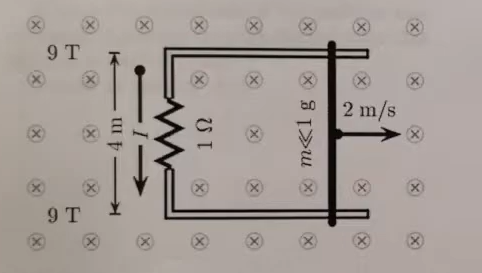
\includegraphics[width=0.5\textwidth]{12.1.PNG}
    \end{center}

    For part (a) use the formula $E=\frac{V}{D}=1.3\times 10^5$ N/C 

    For part (b) use $F_B=F_E = qvB=qE$. SOlving for $v$ we get $6.3\times 10^5$ m/s.
\end{example}

\ex A particle with charge $q$ and mass $m$ is accelerated from rest through a potential difference into a region where both a magnetic field $B$ and an electric field $E$ are present.
The electric and magnetic fields are such that the particle moves in a straight line at constant speed. What is the potential difference through which the particle was accelerated?

\ex \begin{center}
    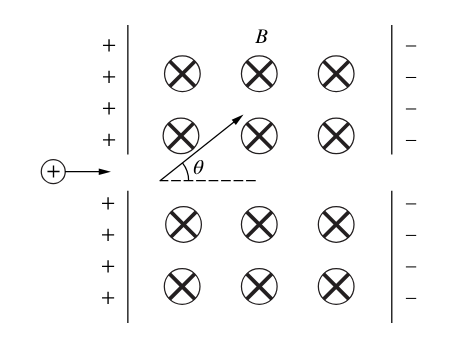
\includegraphics[width=0.5\textwidth]{12.1.1.PNG}
\end{center}
A positively charged particle moves with speed $v$ into the region between two parallel plates. The left plate is positively charged and the right plate is negatively charged to produce an electric field 
with magnitude $E$. A uniform magnetic field $B$ directed into the page exists between the plates. Write a correct equation that could be used to determine the angle $\theta$ relative to the horizontal of the sum of forces on the particle immediately after is enters the region. Gravitational effects can be ignored.

\section{Biot-Savart Law}
The Biot-Savart law defines the magnitude and direction of a magnetic field created by an electric current.
\[ \dd \vec{B} = \frac{\mu_0}{4\pi} \frac{I(\dd l\times \hat{r})}{r^2} \]

The magnetic field vectors around a small segment of a current-carrying wire are tangent to concentric circles centered on that wire.

The Biot-Savart Law can be used to derive the magnitudes and directions of magnetic fields around segments of current-carrying wires.
\[ B_{loop} = \frac{\mu_0 I}{2R} \]

A magnetic field will exert a force on a current-carrying wire.
\[ F_B = \int I(\dd \vec{l}\times \vec{B}) = IlB\sin\theta \]

\begin{example}
    A wire carries a current $I$ in a circular arc with radius $R$ swept through an arbitrary angle $\theta$. Calculate the magnetic field at the center of this arc at point $P$.

    Let $\dd \vec{B}=\frac{\mu_0}{4\pi}\frac{t\dd l\times \vec{r}}{r^2}$.

    Integrating both sides gives us $B=\frac{I\mu_0}{4\pi}\int \frac{\dd l}{r^2}$.
    
    Substituting $l=r\theta \implies \dd l = r\dd \theta$ gives us $B=\frac{\mu_0I}{4\pi}\int_0^{\theta} \frac{\dd \theta}{r}$

    Simplifying this (after taking out $r$ as a constant) gives us $B=\frac{\mu_0I\theta}{4\pi r}$.
\end{example}

\ex \begin{center}
    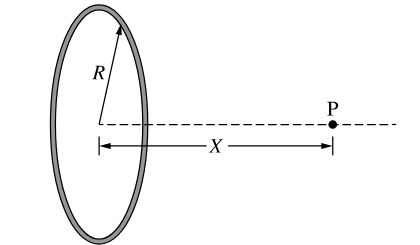
\includegraphics[width=0.5\textwidth]{12.3.PNG}
\end{center}
A circular loop of wire has a radius $R$ and carries a current $I$. Point $P$ is along the central axis of the loop a distance $X$ away from the center of the loop, as shown. What is the magnitude of the magnetic field at point $P$?

\ex \begin{center}
    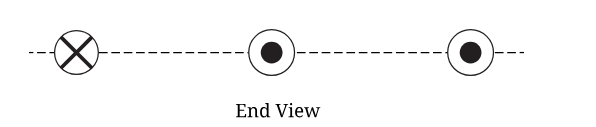
\includegraphics[width=0.5\textwidth]{12.3.1.PNG}
\end{center}
Three long, parallel wires are placed in a horizontal plane and the direction of the current in each wire is as shown. The wire on the left carries current into the page, and the wires in the middle and on the right both carry current 
out of the page. The middle wire is equidistant from the other two wires. The direction of the current in the middle wire is then reversed. How does this affect the direction of the magnetic force exerted on the middle wire?

\section{Ampere's Law}
Ampere's law relates the magnitude of the magnetic field to the current enclosed by an imaginary path called an Amperian Loop.
\[\oint \vec{B}\cdot \dd \vec{l} = \mu_0 I_{enc} \]

Ampere's law can be used to determine the magnetic field near a long, straight current carrying wire.

All solenoids are assumed to very long, with uniform magnetic fields inside the solenoids and negligible magnetic fields outside the solenoids.

Ampere's law can be used to determine the magnetic field inside of a long solenoid.
\[ B_{sol} = \mu_0 nI\]

$n = \frac{\text{Turns}}{\text{Length}} = N/L$

An Amperian loop is a closed path arround a current-carrying conductor.

Ampere's law is the third of Maxwell's equations.
\[ \oint \vec{B} \cdot \dd \vec{l} = \mu_0 I + \mu_0 \epsilon_0 \frac{\dd\phi_E}{\dd t}\]

\begin{example}
    Using Ampere's Law, derive the magnetic field for (a) inside and (b) outside of an infinite cylinder. Be sure to define the Amperian loop. (Assume all currents are distributed uniformly).

    Let's define $r$ as the distance from the center of the cylinder to the Amperian loop and $R$ to be the distance from the center of the cylinder to the surface of the cylinder.

    For part (a) we start with $JA_{loop}=I_{encl}$.

    From this we get that $I_{encl}=\frac{I}{\pi R^2}(\pi r^2)=\frac{Ir^2}{R^2}$.

    We know that $Bl=\mu_0I_{encl}$, so plugging this in gives $B=\frac{\mu_0Ir}{2\pi R^2}$

    For part (b) we have that $Bl=\mu_o I \implies B=\frac{\mu_0 I}{2\pi r}$.
\end{example}

\ex Two long wires are parallel to each other and are 2.0 m apart. Each wire has a current of 3.0 A, but in opposite directions. What is the magnetic field at the midpoint between the wires?

\ex \begin{center}
    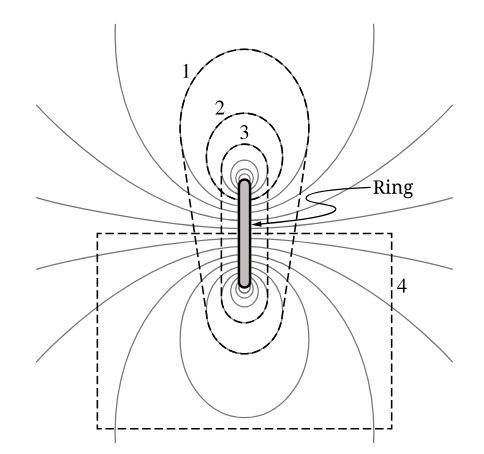
\includegraphics[width=0.5\textwidth]{12.4.PNG}
\end{center}
A circular ring carries and electric current. The magnetic field diagram shown is in a plane that passes through the center of the ring, and which is perpendicular to the plane of the ring.
Four parths 1, 2, 3, and 4, represented by dashed lines, are in the plane of the magnetic field along which the integral $\oint \vec{B}\cdot \dd \vec{l}$ may be evaluated. Which of the paths would yield a result of zero when evaluating this integral?

\end{document}